\section{Introducción}

La Azure Sphere MT3620 development kit es uno de los primeros microcontroladores certificados para utilizar la plataforma Azure Sphere, esta es desarrollada por Microsoft, consiste en una plataforma de aplicación de alto nivel para la comunicación de dispositivos conectados a internet, todo con un enfoque en la seguridad.
\subsection{Azure Sphere}
La plataforma incluye una conexión entre un microcontrolador, un sistema operativo Linux modificado y seguridad continua basada en la nube. La principal apuesta de esta plataforma es la seguridad de alto nivel que proveen. Está diseñada con base en siete propiedades:
\begin{itemize}
	\item 
	\textbf{Actualizaciones de seguridad:} Estos dispositivos se actualizan automáticamente para corregir vulnerabilidades detectadas, esto no requiere intervención del usuario o fabricante.
	\item 
	\textbf{Reporte de errores:} Los dispositivos reportan fallos automáticamente a un sistema en la nube.
	\item
	\textbf{Autenticación sin contraseña:} La plataforma usa certificados firmados; estos se validan por medio de una llave criptográfica, lo que provee una mayor seguridad que el usar contraseñas.
	\item
	\textbf{Niveles de seguridad:} La defensa de esta plataforma es tener varias capas de seguridad, una encima de otra, perfectas para mitigar daños.
	\item
	\textbf{Hardware Seguro:} Cada microcontrolador tiene su identificador único con su propia llave criptográfica, por lo que se usa como un recurso en el que siempre puedes confiar para el sistema de criptografía, lo que normalmente se le llama Root of Trust (RoT).
	\item
	\textbf{Compartimentos dinámicos:}  Limita el alcance de cualquier error. Los microcontroladores de esta plataforma contienen muros físicos que prevén a un error propagarse a otros componentes.
	\item
	\textbf{Pocos componentes críticos a la seguridad:} La mayoría del software se mantiene fuera de la base de computador confiable, solo pocos sistemas que provee Microsoft entran a la seguridad del sistema.
\end{itemize}
\begin{figure}[h]
	\centering
	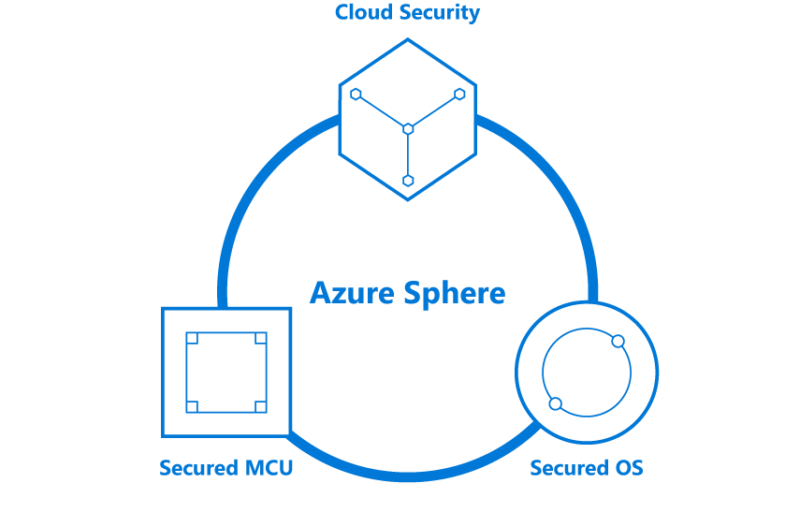
\includegraphics[width=\textwidth,height=\textheight,keepaspectratio]{azuresphere}
	\caption{Descripción gráfica de la plataforma}
\end{figure}